%!TEX root = ../../main.tex


\begin{figure}[!tbp]
\centering
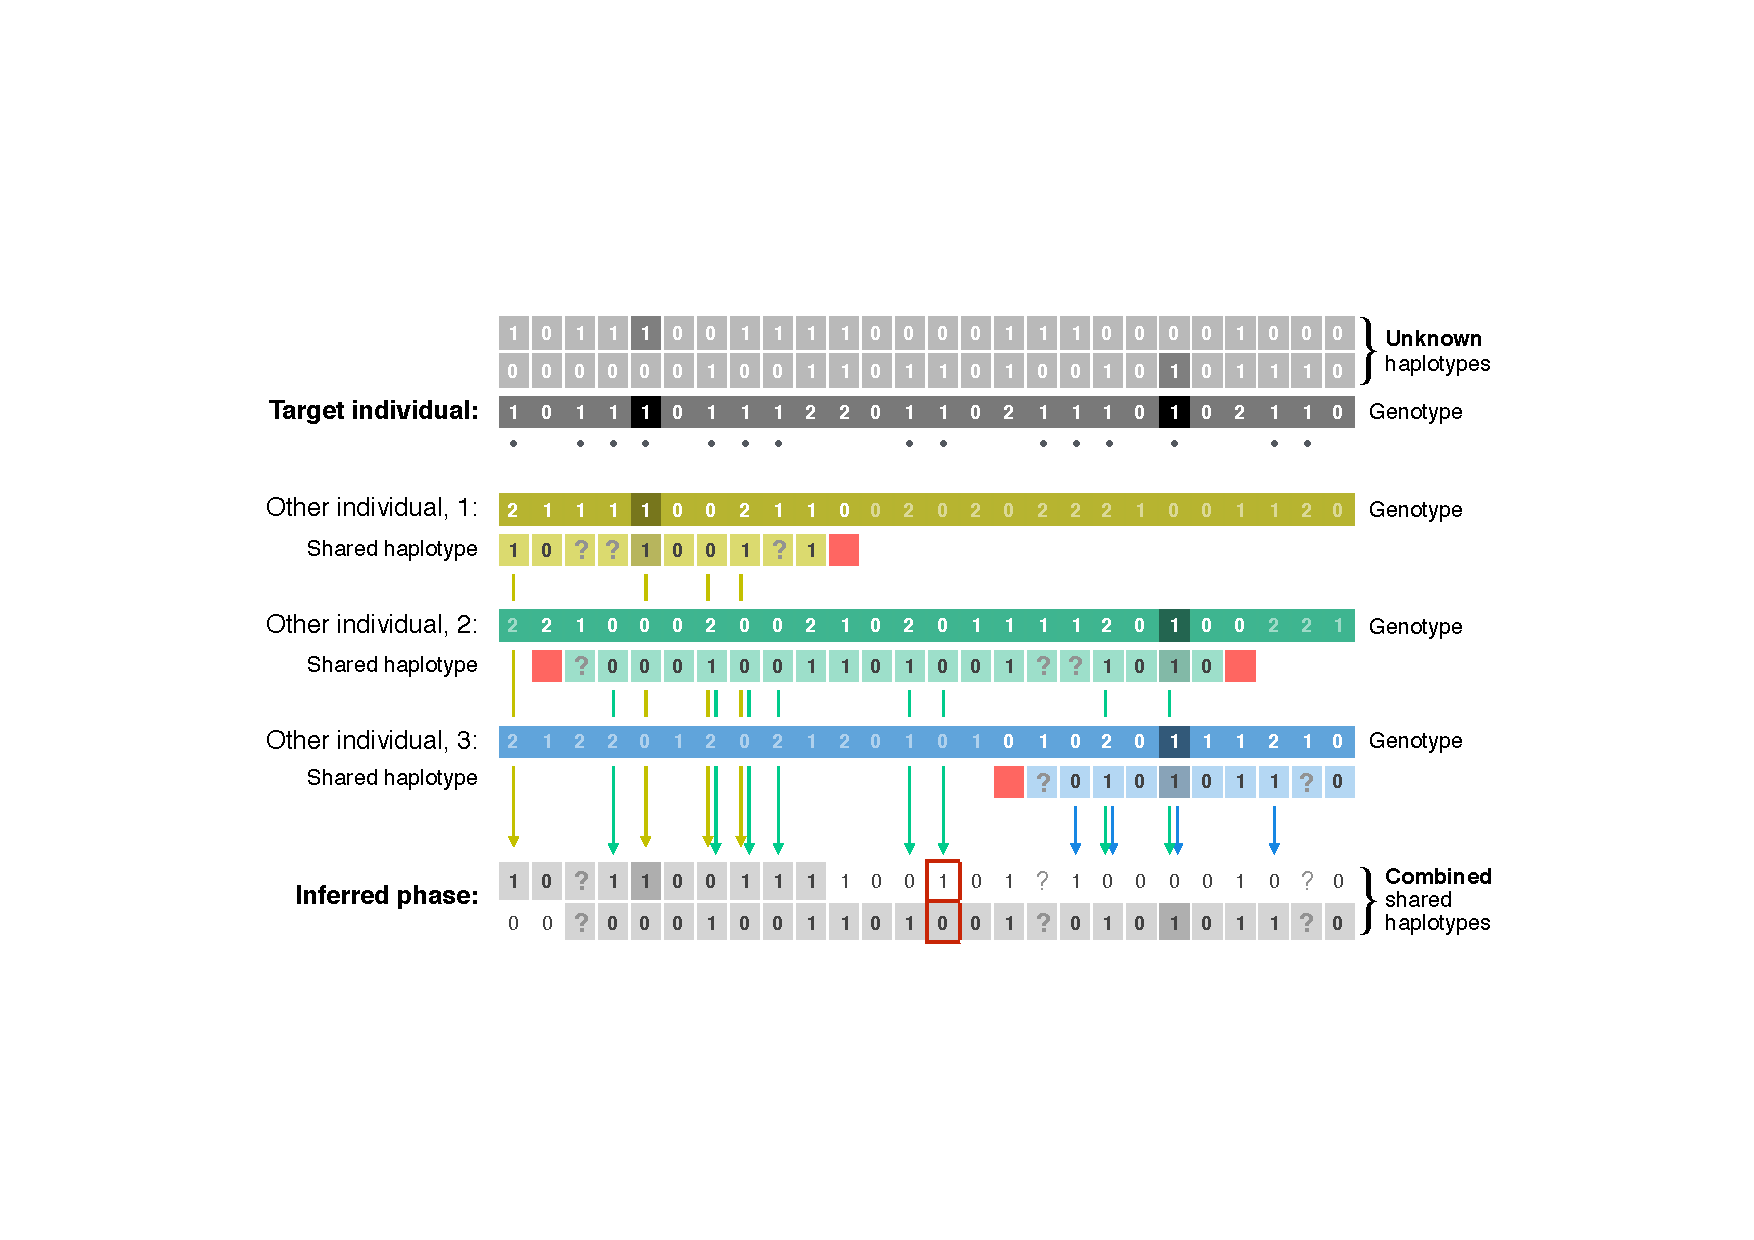
\includegraphics[width=\textwidth]{./img/ch3/info_ibdphasing}
\Caption{Illustration of genotype phasing using detected IBD segments}
{...
% TODO complete caption
Dots below the target genotype indicate heterozygous sites, at which haplotype phase is unknown; haplotypes are already known at homozygous sites, as both haplotypes carry the same allele.

Breakpoints are excluded from inference, because the haplotype cannot be shared at breakpoint positions (\emph{red} blocks).

At positions where both genotypes are heterozygous, the shared haplotype cannot be inferred; indicated by \emph{``?''}.
Note that phase may not be resolved at all sites, even after combination of inferred segments.
Also, singletons may not be phased correctly using this approach; this is illustrated in the figure (\emph{red} outline in inferred phase).}
{fig:info_ibdphasing}
% \vspace{-5pt}
% \hrulefill%
\end{figure}
